\chapter{Практические задания}

\section*{Задание 1}

Составить диаграмму вычисления следующих выражений:
\begin{enumerate}
	\item (equal 3 (abs - 3))
		\begin{figure}[h!]
			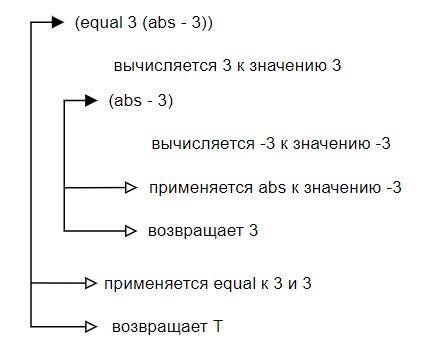
\includegraphics[scale=0.8,left]{img/task1-1}
		\end{figure}
	
	\item (equal (+ 1 2) 3)
		\begin{figure}[h!]
			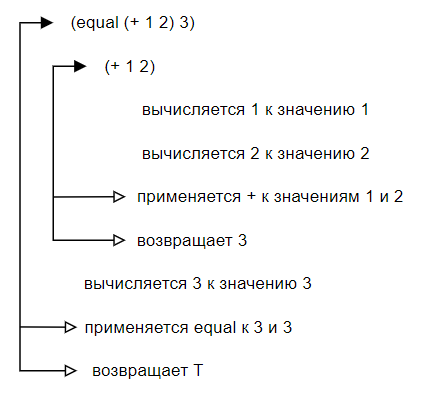
\includegraphics[scale=0.8,left]{img/task1-2}
		\end{figure}
	\clearpage
	\item (equal (* 4 7) 21)
		\begin{figure}[h!]
			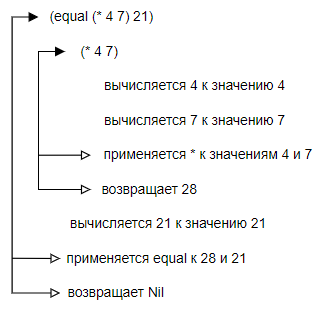
\includegraphics[scale=0.8,left]{img/task1-3}
		\end{figure}
		
	\item (equal (* 2 3) (+ 7 2))
		\begin{figure}[h!]
			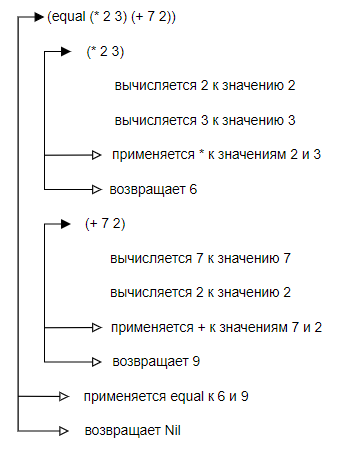
\includegraphics[scale=0.8,left]{img/task1-4}
		\end{figure} 
	
	\clearpage
	
	\item (equal (- 7 3) (* 3 2))
		\begin{figure}[h!]
			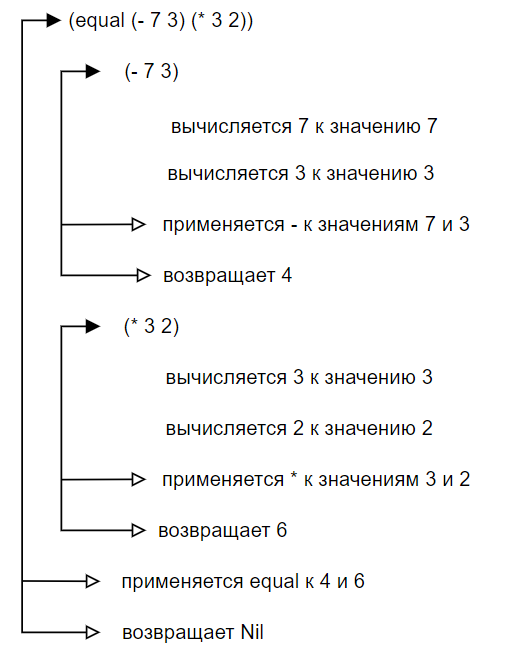
\includegraphics[scale=0.6,left]{img/task1-5}
		\end{figure} 
	
	\item (equal (abs (- 2 4)) 3))
		\begin{figure}[h!]
			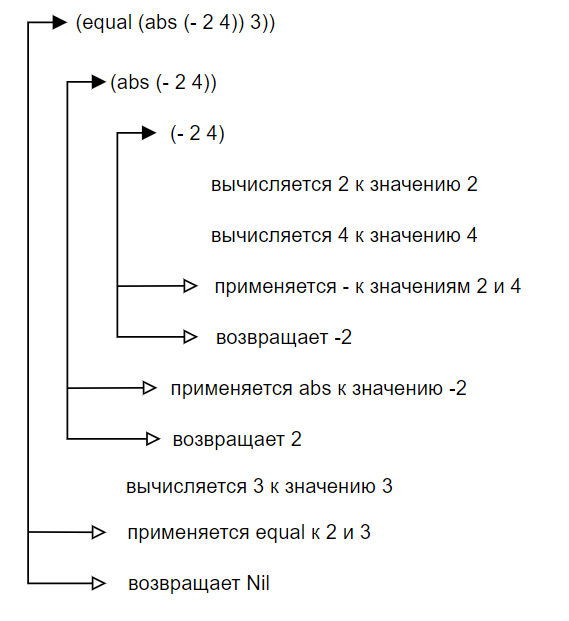
\includegraphics[scale=0.6,left]{img/task1-6}
		\end{figure} 
\end{enumerate}

\section*{Задание 2}
Написать функцию, вычисляющую гипотенузу прямоугольного треугольника по заданным катетам и составить диаграмму её вычисления.

\begin{lstinputlisting}[
	caption={Задание 2},
	label={lst:t2},
	linerange={2-4},
	]{../src/main.lsp}
\end{lstinputlisting}

\begin{figure}[h!]
	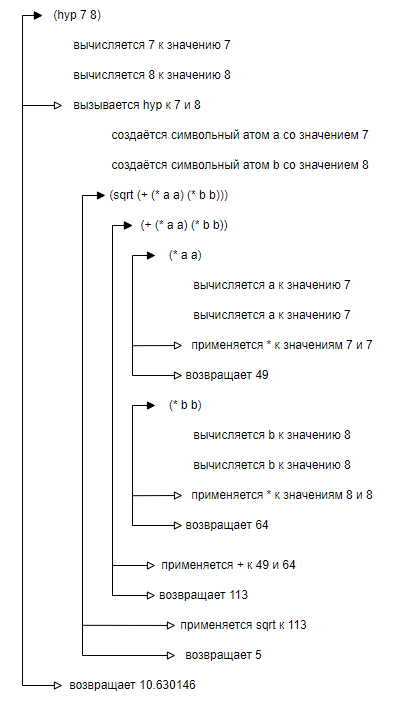
\includegraphics[scale=0.9,left]{img/task2}
\end{figure} 

\section*{Задание 3}
Каковы результаты вычисления следующих выражений?(объяснить возможную ошибку и варианты ее устранения)

\begin{table}[ht]
	\begin{center}
		\begin{tabular}{|c|c|}
			\hline
			\textbf{Выражение} & \textbf{Результат} \\
			\hline
			(list 'a c) & Ошибка: variable c has no value \\
			& Решение: (list 'a 'c) \\
			\hline
			(cons 'a 'b 'c) & Ошибка: too many arguments given to cons \\
			& Решение: (cons 'a (cons 'b 'c)) \\
			\hline
			(cons 'a (b c)) &  Ошибка: undefined function b \\
			& Решение: (cons 'a '(b c))) \\
			\hline
			(list 'a (b c)) & Ошибка: undefined function b \\
			& Решение: (list 'a '(b c)) \\
			\hline
			(cons 'a '(b c))  & (a b c) \\
			\hline
			(list a '(b c)) & Ошибка: undefined function a \\
			& Решение: (list 'a '(b c)) \\
			\hline
			(caddr (1 2 3 4 5)) & Ошибка: 1 is not a function name \\
			& Решение: (caddr '(1 2 3 4 5)) \\
			\hline
			(list (+ 1 '(length '(1 2 3)))) & Ошибка: (LENGTH '(1 2 3)) is not a number \\
			& Решение: (list (+ 1 (length '(1 2 3)))) \\
			\hline
		\end{tabular}
	\end{center}
\end{table}

\section*{Задание 4}
Написать функцию longer\_then от двух списков-аргументов, которая возвращает Т, если первый аргумент имеет большую длину.

\clearpage

\begin{lstinputlisting}[
	caption={Задание 4},
	label={lst:t2},
	linerange={34-40},
	]{../src/main.lsp}
\end{lstinputlisting}

\section*{Задание 5}
Каковы результаты вычисления следующих выражений?

\begin{table}[ht]
	\begin{center}
		\begin{tabular}{|c|c|}
			\hline
			\textbf{Выражение} & \textbf{Результат} \\
			\hline
			(cons 3 (list 5 6)) & (3 5 6)  \\
			\hline
			(cons 3 '(list 5 6)) & (3 LIST 5 6) \\
			\hline
			(list 3 'from 9 'lives (- 9 3)) & (3 FROM 9 LIVES 6) \\
			\hline
			(+ (length for 2 too) (car '(21 22 23))) & Ошибка: variable FOR has no value \\
			\hline
			(cdr '(cons is short for ans)) & (IS SHORT FOR ANS) \\
			\hline
			(car (list one two)) & Ошибка: variable ONE has no value \\
			\hline
			(car (list 'one 'two)) & ONE \\
			\hline
		\end{tabular}
	\end{center}
\end{table}

\section*{Задание 6}
Дана функция (defun mystery (x) (list (second x) (first x))). Какие результаты вычисления следующих выражений?

\begin{table}[ht]
	\begin{center}
		\begin{tabular}{|c|c|}
			\hline
			\textbf{Выражение} & \textbf{Результат} \\
			\hline
			(mystery (one two)) & Ошибка: undefined function ONE \\
			& Решение: (mystery (last '(one two))) \\
			\hline
			 (mystery (last one two)) & Ошибка: variable ONE has no value \\
			 & Решение: (mystery (last '(one two))) \\
			\hline
			(mystery free) &  Ошибка: variable FREE has no value \\
			& Решение: (mystery '(free)) \\
			\hline
			(mystery one 'two) & Ошибка: variable ONE has no value \\
			& Решение: (mystery '(one two)) \\
			\hline
		\end{tabular}
	\end{center}
\end{table}

\section*{Задание 7}
Написать функцию, которая переводит температуру в системе Фаренгейта температуру по Цельсию (defum f-to-c (temp)...).

Формулы:  $c = 5 / 9 * (f - 32.0)$, $f = 9 / 5 * c + 32.0$

\begin{lstinputlisting}[
	caption={Задание 7},
	label={lst:t2},
	linerange={70-72},
	]{../src/main.lsp}
\end{lstinputlisting}

Как бы назывался роман Р.Брэдбери <<+451 по Фаренгейту>> в системе по Цельсию?

Ответ: <<232.78 по Цельсию>>

\clearpage

\section*{Задание 8}
Что получится при вычислении каждого из выражений?

\begin{table}[ht]
	\begin{center}
		\begin{tabular}{|c|c|}
			\hline
			\textbf{Выражение} & \textbf{Результат} \\
			\hline
			(list 'cons t NIL) & (CONS T NIL)   \\
			\hline
			(eval (list 'cons t NIL)) & (T) \\
			\hline
			(eval (eval (list 'cons t NIL))) & Ошибка: undefined function T \\
			\hline
			(apply \#'cons '(t NIL)) & NIL \\
			\hline
			(eval NIL) & NIL \\
			\hline
			(list 'eval NIL) & (EVAL NIL) \\
			\hline
			(eval (list 'eval NIL)) & NIL \\
			\hline
		\end{tabular}
	\end{center}
\end{table}